%%%%%%%%%%%%%%%%%%%%%%%%%%%%%%%%%%%%%%%%%
% Short Sectioned Assignment
% LaTeX Template
% Version 1.0 (5/5/12)
%
% This template has been downloaded from:
% http://www.LaTeXTemplates.com
%
% Original author:
% Frits Wenneker (http://www.howtotex.com)
%
% License:
% CC BY-NC-SA 3.0 (http://creativecommons.org/licenses/by-nc-sa/3.0/)
%
%%%%%%%%%%%%%%%%%%%%%%%%%%%%%%%%%%%%%%%%%

%----------------------------------------------------------------------------------------
%	PACKAGES AND OTHER DOCUMENT CONFIGURATIONS
%----------------------------------------------------------------------------------------

\documentclass[paper=a4, fontsize=11pt]{scrartcl} % A4 paper and 11pt font size

\usepackage[T1]{fontenc} % Use 8-bit encoding that has 256 glyphs
\usepackage{fourier} % Use the Adobe Utopia font for the document - comment this line to return to the LaTeX default
\usepackage[english]{babel} % English language/hyphenation
\usepackage{amsmath,amsfonts,amsthm} % Math packages

\usepackage{lipsum} % Used for inserting dummy 'Lorem ipsum' text into the template
\usepackage{graphicx}

\usepackage{sectsty} % Allows customizing section commands
\allsectionsfont{\centering \normalfont\scshape} % Make all sections centered, the default font and small caps

\usepackage{fancyhdr} % Custom headers and footers
\pagestyle{fancyplain} % Makes all pages in the document conform to the custom headers and footers
\fancyhead{} % No page header - if you want one, create it in the same way as the footers below
\fancyfoot[L]{} % Empty left footer
\fancyfoot[C]{} % Empty center footer
\fancyfoot[R]{\thepage} % Page numbering for right footer
\renewcommand{\headrulewidth}{0pt} % Remove header underlines
\renewcommand{\footrulewidth}{0pt} % Remove footer underlines
\setlength{\headheight}{13.6pt} % Customize the height of the header

\numberwithin{equation}{section} % Number equations within sections (i.e. 1.1, 1.2, 2.1, 2.2 instead of 1, 2, 3, 4)
\numberwithin{figure}{section} % Number figures within sections (i.e. 1.1, 1.2, 2.1, 2.2 instead of 1, 2, 3, 4)
\numberwithin{table}{section} % Number tables within sections (i.e. 1.1, 1.2, 2.1, 2.2 instead of 1, 2, 3, 4)

\setlength\parindent{0pt} % Removes all indentation from paragraphs - comment this line for an assignment with lots of text

%----------------------------------------------------------------------------------------
%	TITLE SECTION
%----------------------------------------------------------------------------------------

\newcommand{\horrule}[1]{\rule{\linewidth}{#1}} % Create horizontal rule command with 1 argument of height

\title{	
\normalfont \normalsize 
\textsc{University of Iowa, Professor Omar Haider} \\ [25pt] % Your university, school and/or department name(s)
\horrule{0.5pt} \\[0.4cm] % Thin top horizontal rule
\huge Databases in OpenEMR \\ % The assignment title
\horrule{2pt} \\[0.5cm] % Thick bottom horizontal rule
}

\author{Junhyuk Kang} % Your name

\date{Sep 27, 2016 ~ Oct 10, 2016 } % Today's date or a custom date


\begin{document}

\maketitle % Print the title

%----------------------------------------------------------------------------------------
%	PROBLEM 1
%----------------------------------------------------------------------------------------
\section{Assignments}
\begin{enumerate}
  \item Show Logdata in csv format
  \item Understand meaning of gacl
  \item How OpenEMR save user's authorities
\end{enumerate}
%----------------------------------------------------------------------------------------
%	PROBLEM 2
%----------------------------------------------------------------------------------------

\section{Answer Steps}

%------------------------------------------------
\begin{itemize}
	\item Tried to find is there any logfile in csv format
	\item There is $C:/Program Files/MySQL/MySQL Server 5.7/Data/mysql/general_log.CSV$
		\begin{itemize}
		\item
		 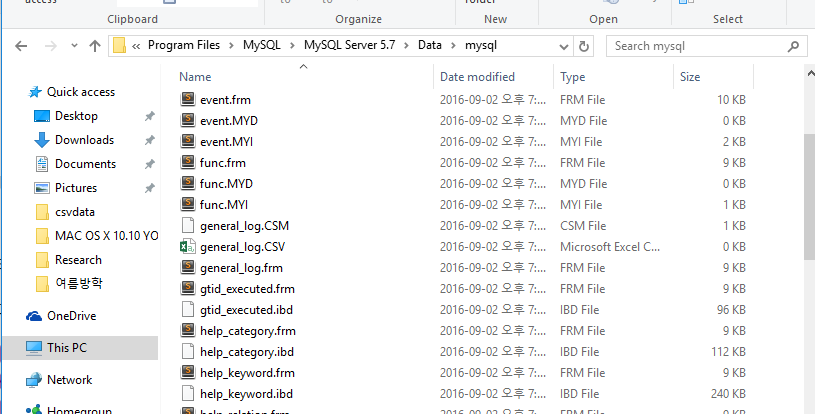
\includegraphics[width = 20cm, height=5cm]{pictures/Emptylogfile.png}
		\end{itemize}
		\begin{itemize}
		\item but it was empty file
		\end{itemize}
	\item Tried to export data from phpMyAdmin
		\begin{itemize}
		\item
		 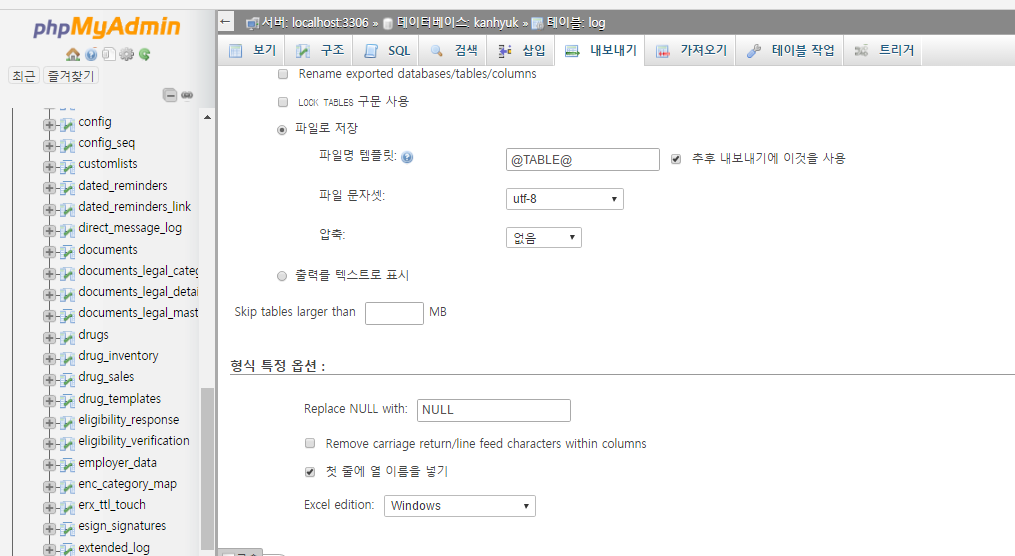
\includegraphics[width = 20cm, height=7cm]{pictures/phpmyadminexport.png}
		\item Chose 'Log' column and export with 'Column names on fisrt low'
		\item it gives all data in one column, used  Data > Text to Columns on Excel to divide those in each columns
		\item
		 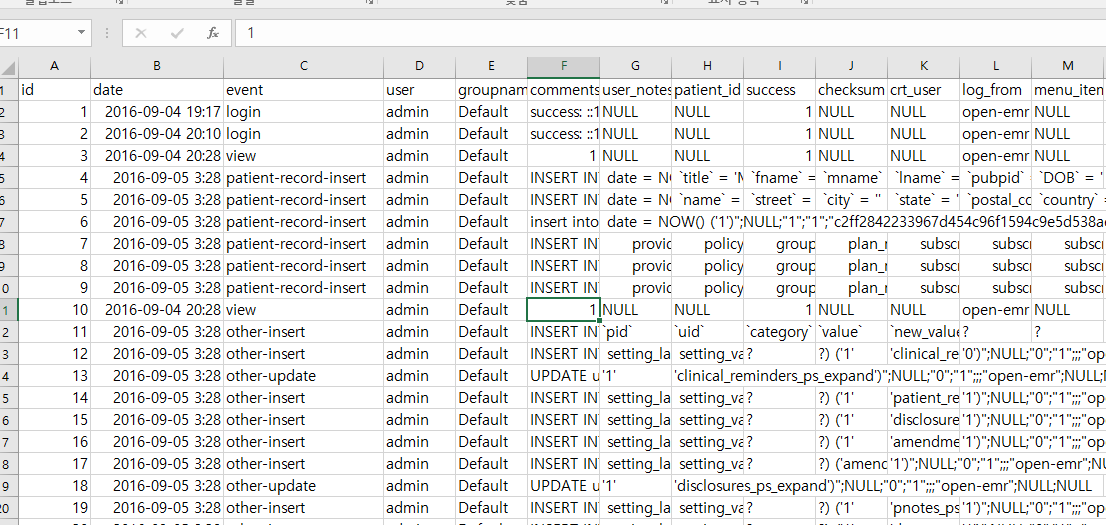
\includegraphics[width = 20cm, height=7cm]{pictures/logfileincsv.png}
		\end{itemize}
	\item 	To understand gacl and OpenEMR's user authority, I export all data from gacl into csv format
	\item  Found sectionvalue, name which gives title of user in tablegaclaco.csv file	
		\begin{itemize}
		\item
		 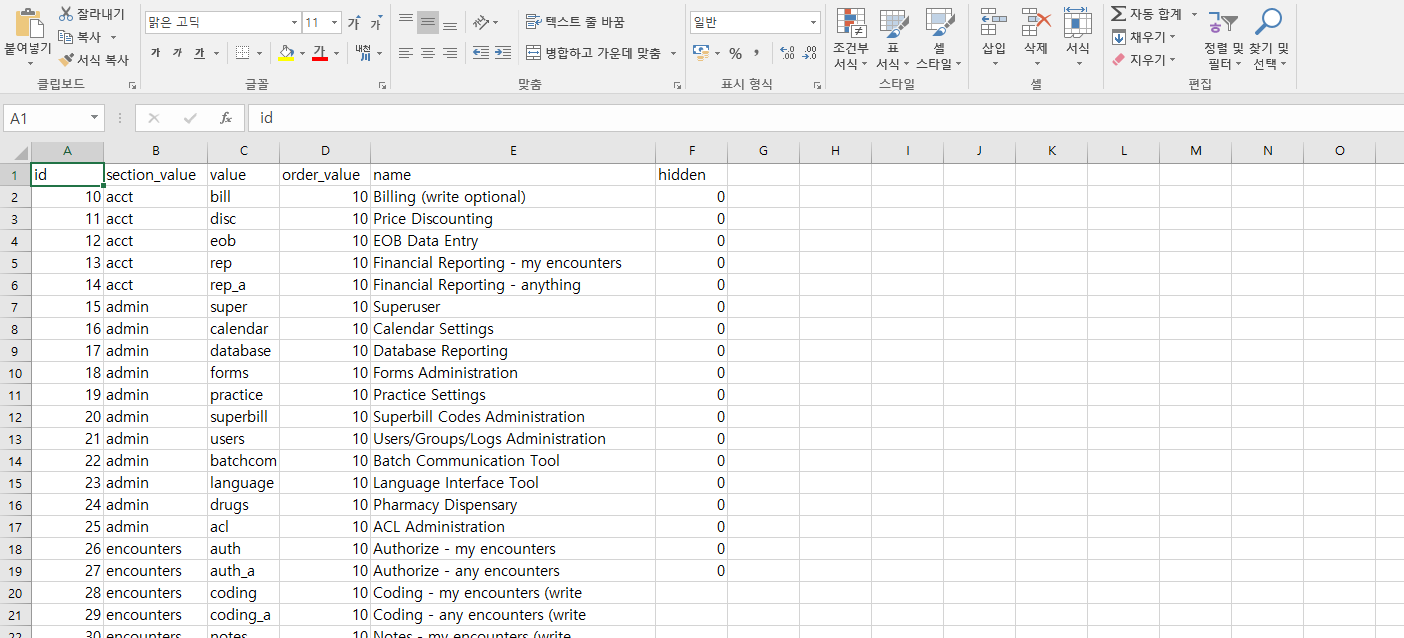
\includegraphics[width = 20cm, height=7cm]{pictures/gacltableauth.png}
		\end{itemize}
	\item Started with looking for keywords(titles of users such as bill, disc, auth, etc inside code), but could not find it
	\item So I tried to find the part where OpenEMR imports the datatable
	\item Searched file name$(gacl_acl)$, and found function $‘add_object_section’$ in $gacl_api.class.php$ file
		\begin{itemize}
		\item
		 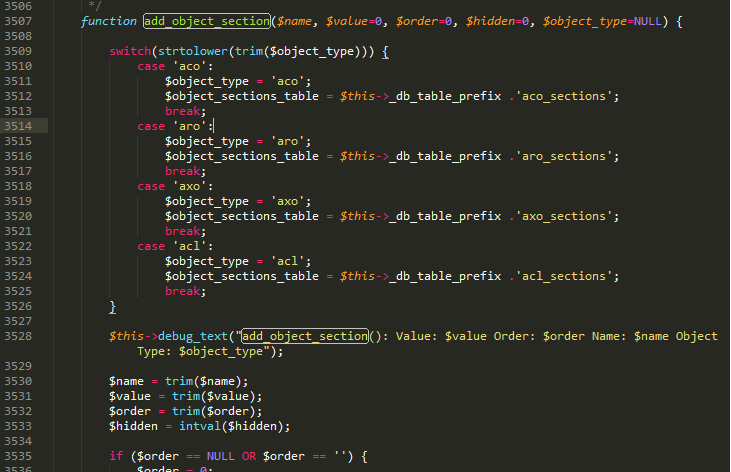
\includegraphics[width = 20cm, height=7cm]{pictures/addobject_func.png}
		\item they import and save table values in objectsectionstable (depends on object type such as aro, aco, axo, acl, it saves into $object_sections_table$)
		\item Realized this file is setting up acl values(add, remove, or modify), not use them
		\end{itemize}
	\item Start to read all the codes from start(except frontend)
		
		\item Found README file on $gacl/test_suite$
		\item 
		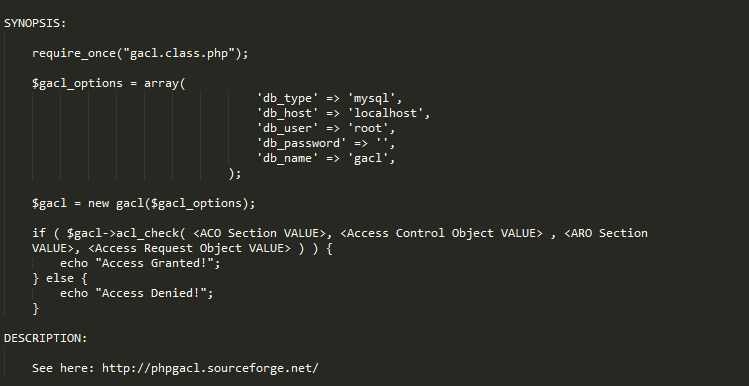
\includegraphics[width = 20cm, height=7cm]{pictures/sypnogacl.png}
		\item Tried to find $acl_check$ function in codes
		\item More info in $http://phpgacl.sourceforge.net/$
		
				\begin{itemize}
				\item ACO(Access Control Objects) =  control what access is available to "requesters"
				\item User definable "Access Request Objects" (ARO). These are objects which request access from an "Access Control Object"
				\item  "Access eXtension Objects" (AXO) grained permissions on each individual item in your application
				\item We can use AXO, ARO with ‘Allow’, ‘Deny’ option 
				\end{itemize}
		\item Found first $acl_check$ in $gacl/admin/templates_c/acl_admin.php$, but it is the part it uses to determine user is admin or not
		\begin{itemize}

		\item
		 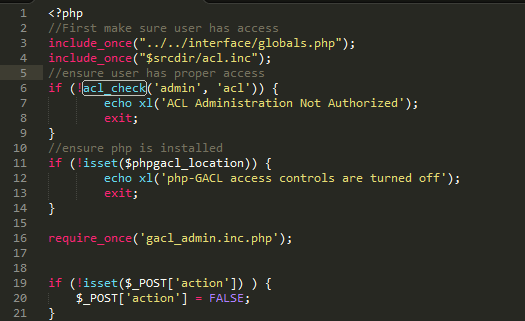
\includegraphics[width = 20cm, height=7cm]{pictures/1staclcheck.png}
		\item
		Realized that every files in $gacl/admin/templates_c start$ with $acl_check$(there is no definition, and it also has $require_once$$('gacl_admin.inc.php')$;, so I tried to find $ (‘gacl_admin.inc.php’)$
		\item 
		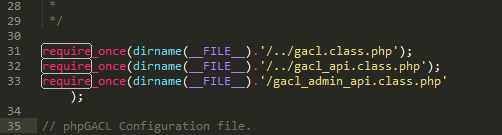
\includegraphics[width = 20cm, height=7cm]{pictures/requires.png}
		\item 
		\end{itemize}
		\item Opened those files one by one
		\item there is a function definition about $acl_check()$ in $gacl.class.php$
realized that $acl_check()$ function is not returning its acl value, and it just determines it is acl or not.(by using array named $‘acl_result’$) and returns only ‘allow’ column.
		\item
		 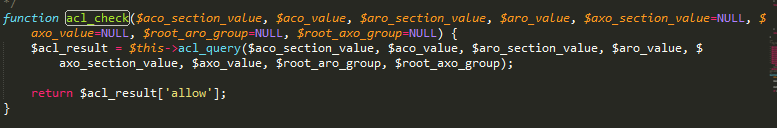
\includegraphics[width = 20cm, height=7cm]{pictures/aclcheckdf.png}
		\item right under $acl_check()$ function, I found $acl_return_value$
		\item
		 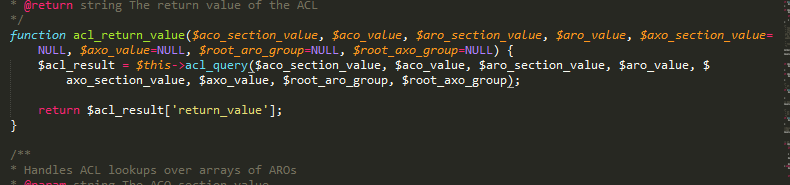
\includegraphics[width = 20cm, height=7cm]{pictures/aclrvdf.png}
		\item It saves $gacl_acl$ values in $acl_result$ array and returns only $ ‘return_value’$ column
		\item So I started to find $acl_result$ array and $acl_return_value()$ function, and $acl_check$, because my hypothesis was
			\begin{itemize}
				\item It will use $acl_check(‘admin’, *)$ to check its role
				\item It will use $acl_return_value()$ to match with strings such as ‘admin’, or ‘physicians’
			\end{itemize}
		\item While searching for the functions and values, found $view_action()$ function in $controllers/C_Document.class.php$
		\item
		 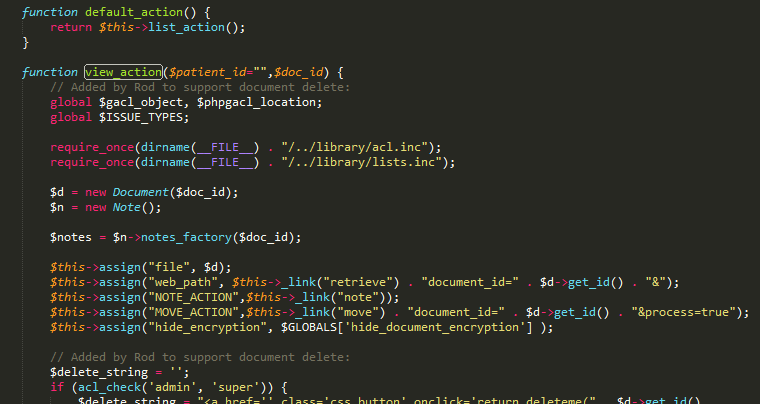
\includegraphics[width = 20cm, height=7cm]{pictures/2ndaclcheck.png}
		\item It uses $acl_check(‘admin’, ‘super’)$ to determine user is administrator or not, and gives authority
		\item I tried to look through codes from start again focused on $acl_check$
		\item Found that $acl_check(‘squads’)$ and $acl_check(‘encounters’)$ in $patient_file/encounter/diagnosis.php$ 
		\item
		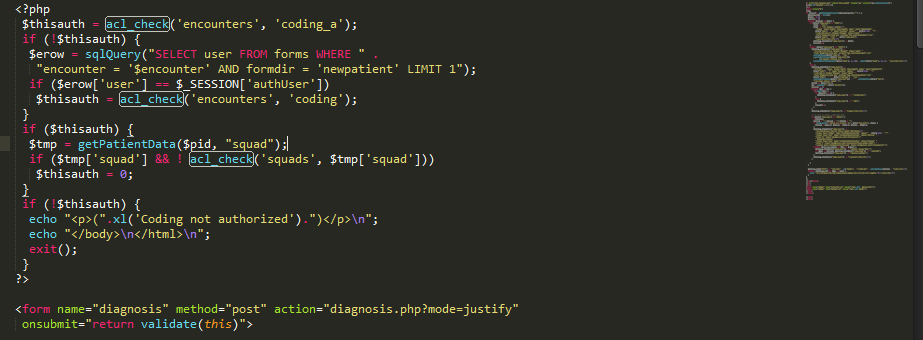
\includegraphics[width = 20cm, height=7cm]{pictures/3rdaclcheck.png}
		\item Also found $acl_check(‘admin’)$ in $patientfile/encounter/forms$, and it gives authority to make new patient only to admin.
		\item
		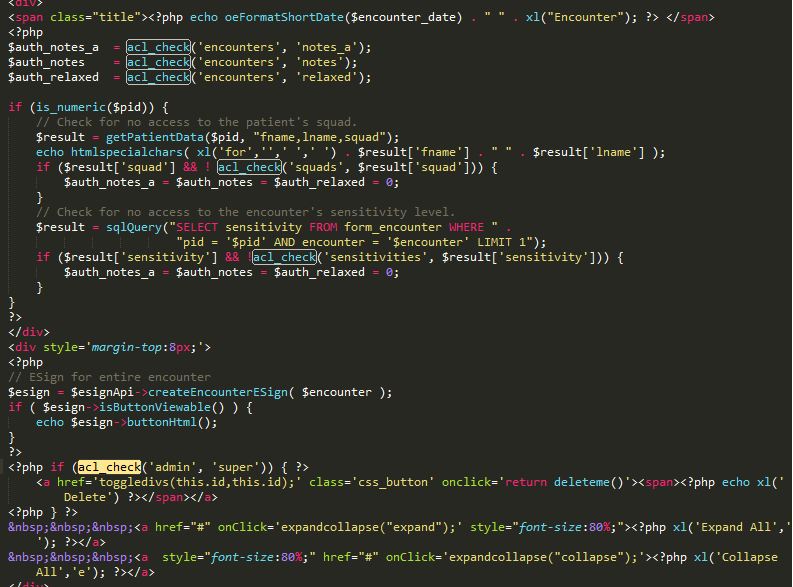
\includegraphics[width = 20cm, height=7cm]{pictures/4thaclcheck.png}
		\item In $patient_file/history/edit_billnote.php$, there is $acl_check(‘acct’, ‘bill’, ‘’, ‘write’)$ which gives authority to edit bill note only to ‘accountant’ to write
		\item
		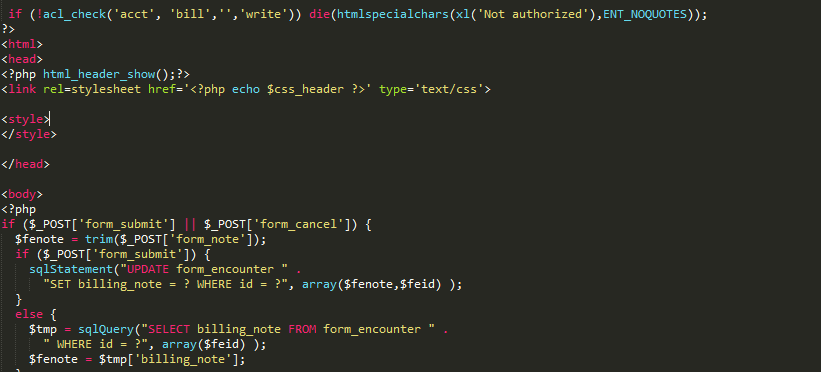
\includegraphics[width = 20cm, height=7cm]{pictures/5thaclcheck.png}
		\item In $patient_file/history/history.php$, $history_full$, $history_save.php$, it has $acl_check(‘patients’, *, * write)$, which makes only patient can write.
		\item
		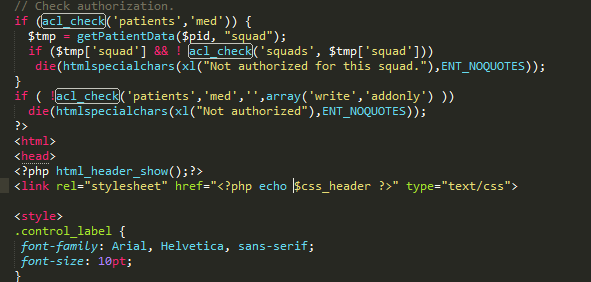
\includegraphics[width = 20cm, height=7cm]{pictures/6thaclcheck.png}
		\item There is $acl_check(‘admin’, ‘super’)$ in $transaction/delete.php$ which gives authority to delete row of data only to administrator
		\item
		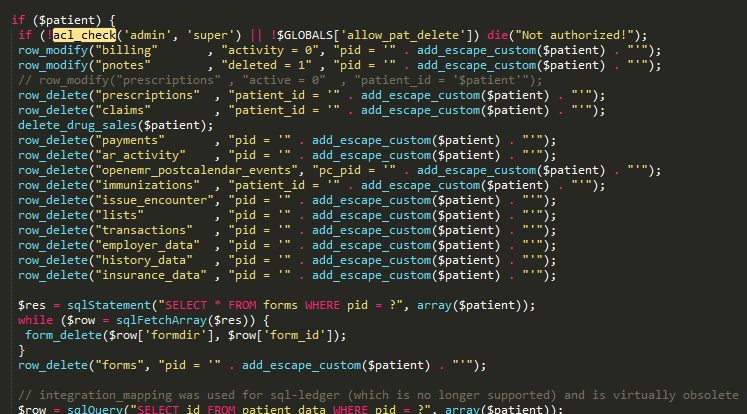
\includegraphics[width = 20cm, height=7cm]{pictures/7thaclcheck.png}
		\item In conclusion, OpenEMR saves user’s authorities in $gacl_aco_sections$, and $table_gacl_acl_sections$. Import those table data in $object_sections_table$, and check the authority by using function $acl_check(values, *, authority)$ (ex, admin, squad… for values, write, view, … for authority)







				
\end{itemize}












\end{document}